\section{在线协同与选择性分流}
\sectionen{Online Coordination and Selective Routing}
\label{sec:online}

\subsection{Motivation}
离线模型给出服务能力，规划器给出下一阶段的资源安排，但请求仍会突发到达。在线层需要持续观察负载，把计划落实到就绪的引擎，并在预测偏差扩大前保护延迟。它同时承担观测预测、快速保护、配置执行、逐请求路由和引擎接力，而不把这些操作留成彼此独立的策略。
\EN{Offline models describe service capacity, and planning proposes the next allocation. Actual requests can still arrive in bursts. The online layer observes demand, applies plans to ready engines, and protects latency before prediction errors accumulate. It coordinates forecasting, protection, resource actions, per-request routing, and engine handoff.}

\subsection{Challenge}
这些操作需要不同的响应速度。新请求必须立即选择去向，风险需要秒级处理，而规划、唤醒和排空可能更慢。与此同时，旧请求仍拥有自己的执行路径和KV；提前发布新阈值、重复启动规划或接纳尚未就绪的实例，都可能使真实负载偏离已评估的方案。
\EN{These operations run at different timescales. Routing needs an immediate decision, protection needs a rapid response, and planning, waking, or draining takes longer. Existing requests still own their execution paths and KV. Premature threshold changes, duplicate planning jobs, or unready instances can invalidate the evaluated workload split.}

\subsection{Insight}
使用一份有效配置连接快慢循环：规划决定资源组合，保护在覆盖范围内提高能力，路由只使用已就绪的路径。新阈值与支撑该分流比例的资源一起发布。请求执行和资源动作异步推进，完成结果与版本回执回到事件循环；降频和缩容则等待稳定条件，而不是在压力刚消失时立即发生。
\EN{Connect the loops through an effective configuration. Planning selects resources, protection increases covered capacity, and routing uses ready paths. Publish a new threshold together with sufficient resources for its workload split. Requests and resource actions run asynchronously and return events. Reducing capacity requires stable observations, not merely the disappearance of one risk signal.}

\subsection{Approach}
\paragraph{接口与状态。}
输入包括请求、性能模型、候选Plan、在途工作和延迟观测；输出包括token流、有效配置、资源动作与完成记录。在线状态区分当前配置、待完成动作和候选计划，同时保留请求绑定的实例与版本。动作完成只说明对应资源已就绪，不能代替请求完成或KV释放证明。
\EN{Inputs are requests, models, candidate plans, active work, and latency observations. Outputs are token streams, effective configurations, resource actions, and outcomes. Track current configuration, pending actions, and candidate plans separately. An action acknowledgement establishes readiness; it does not establish request completion or KV release.}

\paragraph{实例选择与请求接力。}
图~\ref{fig:routing}使用一份\emph{独立的已生效配置示例}，并非上一章规划图的最终输出。8个TP1实例中，I0为P，I1/I2为D，I3--I6为M，I7处于L1。阈值为1024，两个请求均要求128个输出token。短请求输入256，进入在途序列最少的I4；长请求输入2048，进入唯一P实例I0，并从兼容D实例中选择序列更少的I2。P/D配对还必须满足模型、拓扑和请求归属的兼容条件。
\EN{Figure~\ref{fig:routing} starts from an independent effective configuration, not the final output of the planning example. Among eight TP1 instances, I0 is P, I1/I2 are D, I3--I6 are M, and I7 is L1. With threshold 1024, the 256-token request chooses the least-loaded M, I4. The 2048-token request chooses I0 and the less-loaded compatible D, I2.}

P执行原始2048-token输入并产生真实首token $y_1$。代理先向客户端发出$y_1$，再以扩展后的2049-token prompt和127-token剩余预算调用D。D复用原始2048个位置的KV，从$y_1$继续生成$y_2,\ldots,y_{128}$。最终usage仍为输入2048、输出128。逻辑TTFT截止于客户端收到P产生的首token；$y_1$至$y_2$的续接间隙单独观察，不能称为纯KV拷贝时间。输出预算为1时仅在所选M或P执行，不建立远程接力，也不占用D预留。
\EN{P produces the real first token $y_1$. The proxy emits it, then calls D with a 2049-token prompt and a remaining budget of 127. D reuses the original 2048 KV positions and continues the same sequence. Combined usage is 2048/128. TTFT ends when the client receives $y_1$; the continuation gap is separate. One-token outputs use only the selected M or P.}

\begin{algorithm*}[t]
  \caption{ONLINE-COORDINATE}
  \label{alg:online}
  \small
  \begin{algorithmic}[1]
    \State \textbf{procedure} \textsc{Online-Coordinate}()
    \State $C\gets\textsc{Ready-Start}()$; $B\gets C$; $A\gets\varnothing$
    \State \textbf{while} service is running
    \State \hspace{1em}$e\gets\textsc{Next-Event-or-Timer}()$
    \State \hspace{1em}$S\gets\textsc{Observe}(e)$
    \State \hspace{1em}\textbf{if} request result: \textsc{Record}$(e)$
    \State \hspace{1em}\textbf{if} action ACK: $C\gets\textsc{Publish-Ready}(e,A,C)$
    \State \hspace{1em}\textbf{if} new request: \textsc{Spawn-Serve}$(e.request,C)$
    \State \hspace{1em}$R\gets\textsc{Update-Protection}(S)$
    \State \hspace{1em}\textbf{if} slow tick or risk changed
    \State \hspace{2em}\textsc{Coalesce-Plan}$(\textsc{Forecast}(S),C)$
    \State \hspace{1em}\textbf{if} plan ready and \textsc{Still-Valid}$(e,S,C)$
    \State \hspace{2em}$B\gets e.plan$
    \State \hspace{1em}$T\gets\textsc{Stability-Filter}(B,C,S)$
    \State \hspace{1em}$T\gets\textsc{Protect}(T,R)$
    \State \hspace{1em}\textbf{if} \textsc{New-Valid-Target}$(T,C,A)$
    \State \hspace{2em}$A\gets\textsc{Start-Async-Actions}(C,T)$
    \State \hspace{1em}\textsc{Handle-Failed-Actions}$(e,A)$
  \end{algorithmic}
\end{algorithm*}

\begin{figure*}[t]
  \centering
  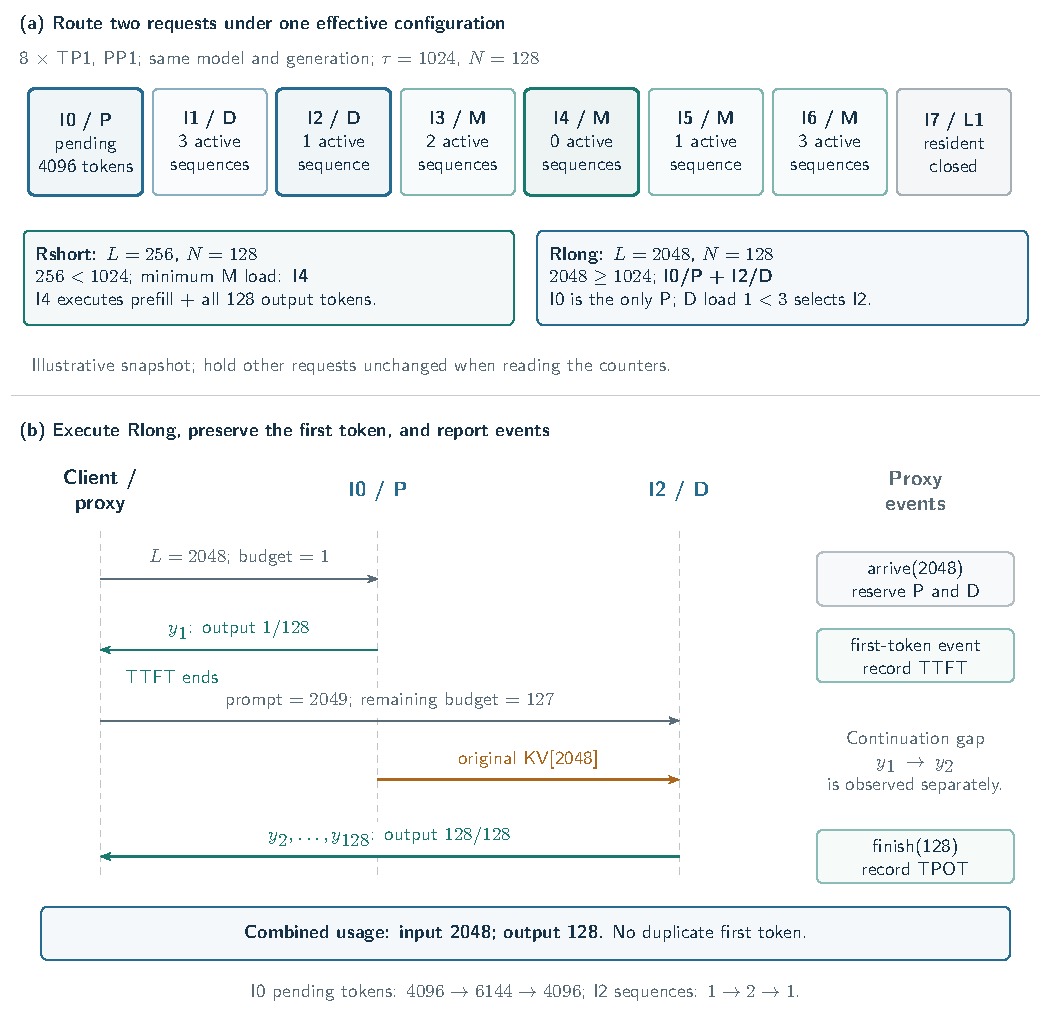
\includegraphics[width=\textwidth]{figures/04-routing.pdf}
  \caption{选择性分流的worked example。(a) 根据角色、阈值和在途负载选择I4或I0/I2；(b) 保留P的首token，延长D的prompt并扣减预算，再向观测端报告到达、首token与完成。示例负载保持其他请求不变；数字不是实测结果，箭头表示逻辑依赖而非精确传输重叠。\\\textit{Worked example of selective routing. (a) Roles, threshold, and active load select I4 or I0/I2. (b) Carry P's first token, extend D's prompt, reduce its budget, and report request events. Other requests are held unchanged in this illustrative snapshot. Values are illustrative; arrows express dependencies rather than exact transfer overlap.}}
  \label{fig:routing}
\end{figure*}

\paragraph{快速保护与稳定回落。}
图~\ref{fig:control}把抽象闭环展开成一次decode压力事件。当前示例周期是1秒检查保护、10秒进行规划，风险变化也能提前请求规划。当TPOT的90分位达到SLO的0.90倍并超过0.80倍保护门限时，先提高活跃实例频率。风险持续则请求唤醒I7作为额外D；pending期间I7不能接收请求，只有就绪回执通过后才形成P1+D3+M4的有效配置。
\EN{Figure~\ref{fig:control} expands the loop into a decode-pressure episode. Example periods are one second for protection and ten seconds for planning, with earlier replanning on risk changes. A TPOT p90 of 0.90 times the SLO crosses the 0.80 protection threshold. Raise clocks first; sustained risk requests another D. I7 remains closed until its readiness acknowledgement is accepted.}

压力消退后，保护期、安静试探和规划稳定条件仍需满足。示例以两个规划窗口确认收缩，再停止I7准入、排空并恢复L1；若压力重现，则恢复所需容量并延长试探窗口。活跃角色复用前也须排空旧工作，或核验新旧负载重叠可行。旧请求不因角色重标记而迁移。图中的频率和阶段仅解释机制，不声称某一时刻已经达到SLO或获得能耗收益。
\EN{After risk clears, respect protection, quiet probes, and stable planning decisions. The example confirms shrinking across two planning windows, then closes, drains, and parks I7. If risk returns, restore capacity and extend the probe. Reusing an active role also requires draining or validating overlapping work. Existing requests are not migrated by relabeling. Frequencies and stages illustrate behavior, not measured gains.}

\begin{figure*}[t]
  \centering
  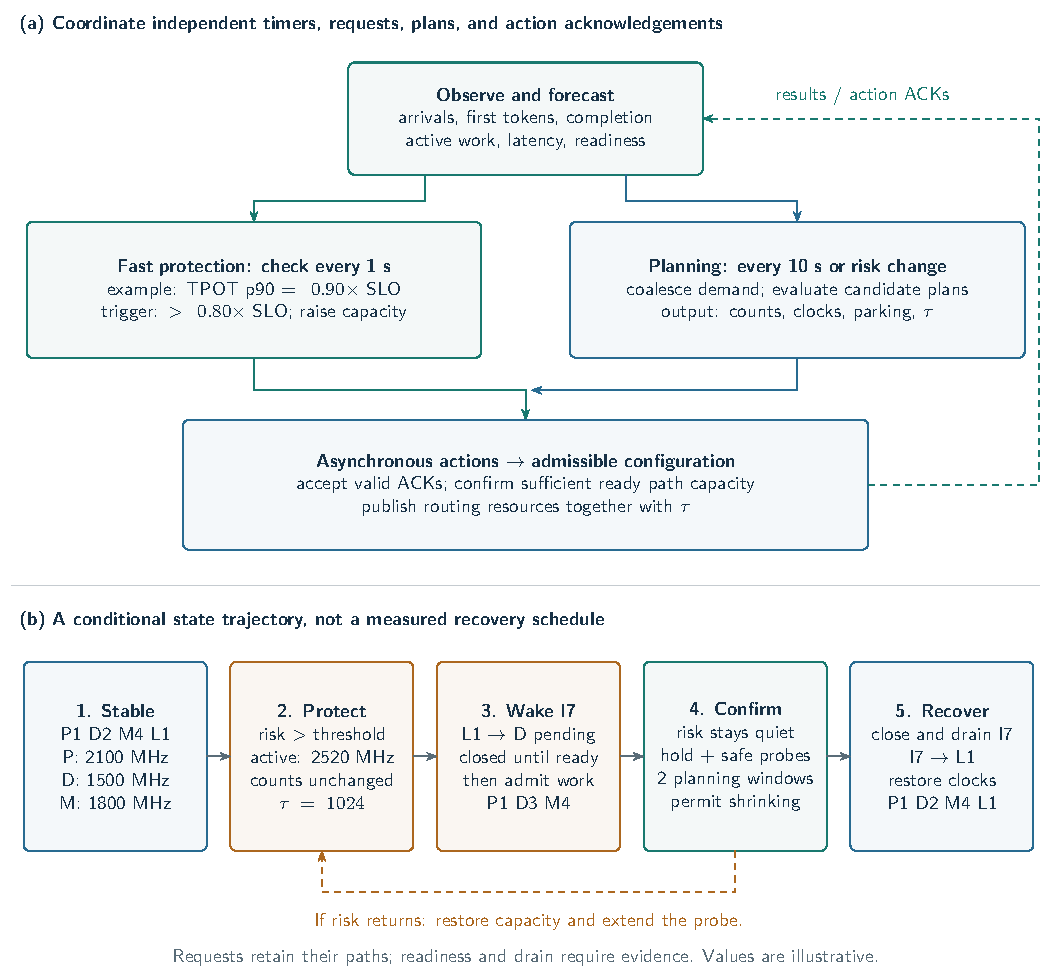
\includegraphics[width=\textwidth]{figures/05-control.pdf}
  \caption{快慢循环的worked example。(a) 具体压力信号和候选Plan经安全执行进入有效配置；新阈值必须具备足够就绪路径容量。(b) 8个实例从P1+D2+M4+L1经升频和唤醒形成P1+D3+M4，之后按保护、稳定和排空条件恢复。阶段不对应固定恢复时刻；频率、负载与状态均为示意。\\\textit{Worked example of online coordination. (a) Pressure and candidate plans reach the effective configuration through safe execution; thresholds require sufficient ready path capacity. (b) Clock escalation and wake-up change P1+D2+M4+L1 to P1+D3+M4, followed by conditional recovery. Stages do not imply fixed recovery times; all values and states are illustrative.}}
  \label{fig:control}
\end{figure*}

\paragraph{事件驱动算法。}
算法~\ref{alg:online}不等待整条请求或资源动作完成；二者通过后台任务返回事件。PLAN调用上一章的选择性分离规划；重复规划请求合并，只保留最新待评估需求。独立定时器在请求持续到达时仍正常触发。接受结果前检查规划编号与配置版本，接受资源回执前检查动作编号，过期结果不得覆盖新配置。
\EN{Algorithm~\ref{alg:online} never waits for an entire request or resource action. Background work returns events. PLAN invokes the preceding planning method; duplicate requests are coalesced around the latest demand. Independent timers continue under traffic. Validate planning identifiers and configuration versions, and validate action identifiers before accepting acknowledgements. Stale results cannot replace newer configurations.}



\textsc{Publish-Ready}只发布可准入的配置：新阈值须和足够的M/P/D路径容量一起生效；过渡期保持旧配置或核验中间配置，必要时限制准入。\textsc{Protect}保持阈值及既有容量下界，只在测量覆盖内升频或扩充角色容量；若改变分流规则则重新评估。稳定条件不能阻挡紧急保护升级。规划与动作异步并不意味着整个集群原子切换。
\EN{Publish-Ready installs admissible configurations only: a new threshold requires sufficient M/P/D capacity. Retain the old configuration or validate intermediate states, limiting admission if needed. Protect preserves the threshold and capacity floor while increasing covered clocks or capacity. Routing changes need re-evaluation. Stability gates must not block urgent protection; asynchronous actions do not imply an atomic fleet-wide switch.}

\begin{algorithm}[H]
  \caption{SERVE: asynchronous request helper}
  \label{alg:serve}
  \small
  \begin{algorithmic}[1]
    \State \textbf{procedure async} \textsc{Serve}$(r,C)$
    \State $p\gets\textsc{None}$; \textbf{try}
    \State \hspace{1em}$p\gets\textsc{Validate-and-Reserve}(r,C)$
    \State \hspace{1em}\textbf{if} $p=\textsc{None}$: \textbf{raise} unavailable
    \State \hspace{1em}\textbf{if} M or $N=1$: $z\gets\textbf{await}\ \textsc{Single}(p,r)$
    \State \hspace{1em}\textbf{else}: $z\gets\textbf{await}\ \textsc{Carry-and-Decode}(p,r)$
    \State \textbf{catch} failure: $z\gets\textsc{Failed}(failure)$
    \State \textbf{finally}: \textsc{Report-and-Resolve-Ownership}$(r,z,p)$
  \end{algorithmic}
\end{algorithm}

算法~\ref{alg:serve}中$N$为请求的输出预算，派发时再次检查准入和有效版本。短请求的完整输出与长请求的首token接力，都在各自异步任务内执行。成功、拒绝、失败和取消仅报告一次；未确认的KV或传输资源继续保留归属并隔离，客户端断开不能自动视为资源释放。
\EN{In Algorithm~\ref{alg:serve}, $N$ is the output budget. Recheck admission and version at dispatch. Single-engine output and PD continuation run in their own asynchronous tasks. Report each outcome once. Retain ownership and quarantine uncertain KV or transfer resources; client disconnection is not evidence of release.}

\implnote{以上版本回执与异步协调是目标设计的组织方式。当前主控制器排空主要依据代理的prefill与sequence计数，尚不等于已证明原生KV及传输资源清零。当前PD接力受限于token-ID输入、greedy、固定输出预算以及同TP、PP1；这些限制不应被写成已支持任意采样或跨TP迁移。}{The acknowledgement-driven organization is the target design. Current main-controller drain primarily uses proxy prefill and sequence counts; this does not prove native KV and transfer resources are empty. Current PD carry requires token IDs, greedy sampling, a fixed output budget, and matching TP with PP1. It does not establish arbitrary sampling or cross-TP migration.}
